\documentclass[12pt]{article}
\usepackage[margin=1in]{geometry}
%\usepackage{hyperref}
\usepackage{amsmath}
\usepackage{graphicx}% http://ctan.org/pkg/graphicx
\usepackage{systeme}
%% tables
\usepackage{booktabs}
\usepackage[table,xcdraw]{xcolor}
\usepackage{float}

%% Make red text
\newcommand{\com}[1]{\textcolor{red}{ #1}}

%\linespread{2}

\usepackage[authoryear]{natbib}


\usepackage{tikz}
\tikzset{
  int/.style={circle, draw, fill=blue!20, minimum size=3em},
  init/.style={pin distance=1.2cm,pin edge={loop,thin,black}}
}
\usetikzlibrary{arrows,automata}

\pagenumbering{arabic}

\newcommand{\XX}{\ensuremath{25}} % number of methods

\newcommand{\xxsir}{\ensuremath{9}} % number of SIR methods

\newcommand{\rr}{\ensuremath{\mathcal{R}_0}}

\setlength{\itemsep}{0pt}






\begin{document}

%%% draw a tree
\tikzset{
  treenode/.style = {shape=rectangle, rounded corners,
                     draw, align=center,
                     top color=white, bottom color=blue!20},
  root/.style     = {treenode, font=\Large, bottom color=red!30},
  env/.style      = {treenode, font=\ttfamily\normalsize},
  dummy/.style    = {circle,draw}
}




\title{An overview of $\xxsir$ methods to estimate $\rr$ from the SIR model and comments on more complex models}
\author{ Department of Statistics, Carnegie Mellon University}
\date{\today}
\maketitle

% \tableofcontents


\section{Introduction}\label{sec:intro}
What has been called ``arguably the most important quantity in the study of epidemics'' \citep{Heesterbeek2002},  $\mathcal{R}_0$, the reproduction number (by convention pronounced ``R-naught'') is a persistently elusive quantity for epidemic modelers to estimate.  As defined by \citet{anderson1992}, $\rr$ is the ``the average number of secondary infections produced when one infected individual is introduced into a host population where everyone is susceptible.''  $\rr$, in some ways, summarizes an entire outbreak of a disease; it  is used to assess whether a disease epidemic will occur.  Additionally, it describes what percentage of the population needs to be vaccinated to avoid such an epidemic.  Despite a clear definition of $\rr$, epidemiologists have struggled to create a standard  estimator for $\rr$  \citep{hethcote2000}.  A major issue in estimating $\rr$ is that the quantity is a \textit{property of the model}, meaning that $\rr$ is dependent not only on the usual noise that comes with statistical modeling but also on a variety of assumptions on how researchers assume a disease is transmitted through a population.

To elaborate on $\rr$ being the property of the model, we first need to introduce the concept of the ``SI-framework,'' which was pioneered by Kermack and McKendrick in the 1920s \citep{getz2006}.   Here, S and I are known as compartments where S stands for ``susceptible'' and I for ``infectious.'' Infectious disease models then specify how individuals move from the S compartment to the I compartment.  Often, ancillary compartments are added such as R, which stands for recovered or dead, or E, which stands for exposed but not yet infectious.  The estimate of $\rr$ from a SIR model will not be directly comparable to the estimate of $\rr$ from a SEIR model, for example.  The difficulties of estimating $\rr$ are summarized and expanded upon by \cite{li2011}.   As a result of $\rr$ being a property of the model, we limit our review to methods for estimating $\rr$ for the SIR model introduced by \cite{Kermack700}.

Even when limiting $\rr$ estimates to those from SIR models, estimation is still difficult.  Problems include mathematical versus statistical methods (i.e. solving for $\rr$ versus estimating $\rr$), the number of observations used to estimate $\rr$ (i.e. time), boundary cases of infection and recovery rates, population size, initial SI ratio, and restrictive assumptions placed upon the noise.  These are all issues for estimating single points, to say nothing of confidence or credible intervals (CI).

We review $\xxsir$ methods for estimating $\rr$.  We note that these methods are not exhaustive but are chosen due to their impact and use in epidemiology.  We find that these methods also help to highlight the problems discussed above.  In addition to making a point estimate of $\rr$, we are particularly interested in the hypothesis  $H_0: \rr > 1$, as a value greater than 1 indicates an outbreak of a disease.  As such, we discuss techniques for estimating CIs for each of the different methods.  These techniques include, the delta method, block bootstrap, and the posterior distribution.

Following, we present a series of simulations in which we examine each of our $\rr$ estimation methods.  Within these simulations, we vary the number of observations used to estimate $\rr$, infection and recovery rates, the total population size, initial SI ratio, and several assumptions about the noise.

We find that...

Finally, we discuss our recommendations in estimating $\rr$ for the SIR model.  Afterwards, we comment on how these recommendations extend to more complex models and how many of the problems with estimating $\rr$  become exacerbated with the increase in complexity.


The rest of this manuscript is organized as follows.  In Section \ref{sec:r0}, we briefly discuss the origin of $\rr$.  In Section \ref{sec:sir-intro}, we introduce the SIR model as described by \cite{Kermack700}.  In Section \ref{sec:methods}, we overview the $\xxsir$ methods for estimating $\rr$. In Section \ref{sec:ci}, we discuss how to estimate CIs for each of the $\xxsir$ methods.  Following in Section \ref{sec:sim-res}, we present the results of our simulations.  Finally, in Section \ref{sec:discussion}, we provide final analysis of estimating $\rr$ for the SIR model and offer comments on how these conclusions extend to more complex models.


\section{Origins of $\rr$}
\label{sec:r0}

The origins of $\rr$ are tied to the survival function.  This function, which originates from the field of demography in the late 1800s, describes how many female offspring a woman is expected to produce in her lifetime \citep{dietz1993estimation}.  In demography, we have
\begin{align}\label{eq:surv}
\rr = \int_0^\infty p(a) \beta(a) da
\end{align}
where $p(a)$ denotes the probability of a woman surviving to age $a$ and $\beta(a)$ the rate of an individual of age $a$ giving birth to a  girl.   This interpretation also explains the origins of the name of $\rr$.  The concept of the reproduction number was later imported to the field of epidemiology by MacDonald and Smith \citep{dietz1993estimation}.  Analogously in epidemiology, $p(a)$ is the age of a disease, and $\beta(a)$ is the infection rate.

This is the chronologically first, and in many ways, the most direct method to estimate $\rr$.  As we see here, the SIR model is not even mentioned in this derivation.  The premise of this whole paper is based upon the fact that estimating $\rr$ from the survival function in Equation \eqref{eq:surv} is a difficult task.  It is due to this difficulty that other estimates even exist and why we must discuss $\rr$ as a property of the SIR model.


\section{Kermack and McKendrick's SIR Model}
\label{sec:sir-intro}

The SIR model introduced by \cite{Kermack700} is a compartment model, where individuals move from susceptible, to infectious, and finally recovered states.  We make four essential assumptions,
\begin{enumerate}
\item The compartments are discrete and have no overlap.
\item The transition of objects into and out of compartments is described by a set of known equations, possibly dependent on unknown parameters.
\item The populations mix homogeneously
  \item The number of objects in each compartment at time $t=0$ is known
  \end{enumerate}  


Another common assumption for compartment models, is the law of mass action, a property borrowed from chemistry which says that the mass of the product is proportional to the mass of the reactants.  In epidemiology, this means that the proportion of new infections is proportional to the current  number of susceptible \citep{anderson1992}.  Therefore, the flow of objects from one compartment to another may be dependent on the percentage of objects within one or many of the compartments. 


In this particular  SIR model, $N$, the number of individuals is constant, as we see no arrows pointing away from the three nodes in Figure \ref{fig::sir}. Simple adaptations of the SIR model can include birth and death rates, which may correspondingly change the derivation of $\rr$ (for further discussion, see Section \ref{sec:discussion}). The parameters  $\beta$ and $\gamma$ have epidemiological meaning.  Here, $\beta$ is the average infection rate and $\gamma$ is the average recovery rate.  The movement of individuals from one compartment to another is represented through the ordinary differential equations below.  Both $\beta$ and $\gamma$ are constrained to be between $0$ and $1$.  Throughout, we use $X$, $Y$, and $Z$ for stand-ins for the ODEs for $S$, $I$, and $R$, respectively, to avoid any confusion with $\rr$.
\begin{align}
\systeme{\frac{dX}{dt} = -\frac{\beta XY}{N}, \frac{dY}{dt} = \frac{\beta XY}{N} - \gamma Y, \frac{dZ}{dt} = \gamma Z}. \label{eq:sir}
\end{align}
In words, susceptible individuals become infected at a rate that is proportional to the percentage of infected individuals multiplied by $\beta$, the infection rate, and the number of susceptible individuals.  Infectious individuals recover at a rate of $\gamma$ multiplied by the number of infected individuals.


The SIR model is represented graphically in Figure \ref{fig::sir}. 
\begin{figure}[h]
\centering
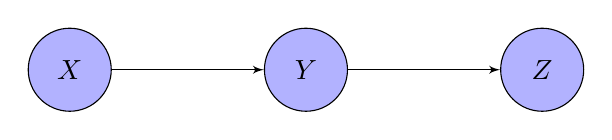
\begin{tikzpicture}[node distance=3cm,auto,>=latex',every node/.append style={align=center}]
    \node [int,  fill = white!70!blue] (a)              {$X$};
    \node [int,  fill = white!70!blue]           (c) [right of=a] {$Y$};
    \node [int,  fill = white!70!blue] (e) [right of=c] {$Z$};
    \path[->, auto=false] (a) edge node {} (c)
                          (c) edge node {} (e) ;

\end{tikzpicture}
\caption{Depiction of a SIR model where $X=S, Y=I,$ and $Z=R$.  One can only get the disease once in this model.}\label{fig::sir}
\end{figure}
An outbreak occurs if the rate of change of infectious individuals is positive,
\begin{align*}
  \frac{dY}{dt} &> 0 \\
  \frac{\beta X Y}{N}  - \gamma Y &> 0 ,\\
  Y \left ( \beta \frac{X}{N} - \gamma \right ) & > 0\\
   \frac{\beta}{\gamma} &> \frac{N}{X}.
\end{align*}
That is,  the rate of new infections is greater than the rate of recovery.  So as long as the number of susceptibles is large, $\frac{X}{N} \approx 1$, then an outbreak will occur if $\rr >1$,
\begin{align*}
  \rr \overset{def}{=} \frac{\beta}{\gamma} > 1.
  \end{align*}
  In order to incorporate randomness, we add noise, namely,
  \begin{align}\label{eq:sir-noise}
    X_{obs}(t) &= X(t) + \epsilon_{X,t}\\
    Y_{obs}(t) &=  N - X_{obs}(t) -Y_{obs}(t)  \nonumber\\
    Z_{obs}(t) &= Z(t) + \epsilon_{Z,t}. \nonumber
  \end{align}
We are assuming the observations are generated based on the deterministic ODEs presented in Equation \ref{eq:sir} with the addition of time ($t=0, 1, \dots, T$0) and compartment dependent noise $\epsilon_{X,t}$ and $\epsilon_{Z,t}$.  Since, $N$, the total population, is constant, then $Y_{obs}$ is adjusted accordingly.

In summary, when we discuss estimators for $\rr$ for the SIR model, we mean to say we are forming an estimator of $\rr$ from the given set of data in Eq. \ref{eq:sir-noise},
\begin{align*}
\textnormal{data} = \left \{\left (X_{obs}(t), Y_{obs}(t), Z_{obs}(t) \right ) : t=0, 1, \dots, T\right \}.
  \end{align*}.
  
\section{Overview of $\xxsir$ methods to estimate $\rr$ for the SIR model}
\label{sec:methods}

In this section, we describe the $\xxsir$ methods in detail.  

\subsection{Least Squares ($\beta$, $\gamma$) (LS)}\label{least-squares-beta-gamma}
The first approach to estimate $\rr$ in the SIR model is to minimize the joint mean square error for the data collected at each time point and use the plug-in estimator found in Equation \ref{eq:sirls}.  In particular, we find

\begin{align*}
(\hat{\beta}, \hat{\gamma} )&=\arg \min_{\beta, \gamma} \sum_{t} \left [ \left (X_{obs}(t) - X(t)\right )^2 + \left ( Z_{obs}(t) - Z(t) \right )^2 \right ]
\end{align*}
Then  the estimate for $\rr$ is given by Equation \ref{eq:sirls},
\begin{align}\label{eq:sirls}
  \hat{\rr}= \frac{\hat{\beta}}{\hat{\gamma}}.
  \end{align}


\subsection{Reparametrized Least Squares ($\rr$, $\gamma$) (ReLS)}\label{reparametrized-least-squares-rux5f0-gamma}

In the previous method (Section \ref{least-squares-beta-gamma}), we estimated $\beta$ and $\gamma$ and then estimated $\rr$.  However, it is possible to directly estimate $\rr$ if we reparametrize the ODEs in Equation \eqref{eq:sir} directly with \(\rr\) and \(\gamma\), using the relation $\rr = \frac{\beta}{\gamma}$,

\begin{align*}
  \left \{
  \begin{array}{cl}
    \frac{dX}{dt} &= - \rr \gamma Y \frac{X}{N}\vspace{.5em}\\
    \frac{dY}{dt} &=  \rr \gamma Y \frac{X}{N}  - \gamma Y\vspace{.5em} \\
    \frac{dZ}{dt} &=  - \gamma Y 
  \end{array}
  \right . .
  \end{align*}
We find
\begin{align*}
(\hat{\rr}, \hat{\gamma} ) &= \text{argmin}_{\beta, \gamma} \sum_{t} \left [ \left (X_{obs}(t) - X(t)\right )^2 + \left ( Z_{obs}(t) - Z(t) \right )^2 \right ]
\end{align*}
We use the $\hat{\rr}$ directly from the above estimation process, which again can be done with gradient descent or another optimization process.



\subsection{Linear Model Approximation (LMA)}\label{linear-model-approximation-degree-10}

The SIR ODEs in Eq. \ref{eq:sir} have no known closed form solution, and so we are already using approximations using numerical integration, albeit small ones.  In addition to this, data collected from real diseases are typically very noisy to begin with.  \cite{chang2017} discovered that an SIR model may be well approximated by a linear model.  We use this approach here to estimate $\rr$.

Specifically, we estimate two linear polynomials in \(t\) with degree \(K= 10\) to \(X_{obs}\)
and \(Y_{obs}\) using least squares to find the coefficients $\{(\hat{x}_k,
\hat{y}_k)\}_{k=1, \dots, K}$,
\begin{align*}
\hat{X}(t) &= \sum_{k=0}^K \hat{x}_k t^k\\
{\hat{Y}}(t) &= \sum_{k=0}^K \hat{y}_k t^k
\end{align*}
Then, we estimate the derivatives as
\begin{align*}
\hat{X}^\prime(t) &= \sum_{k=1}^K k \hat{x}_k t^{k-1}\\
\hat{Y}^\prime(t) &= \sum_{k=0}^K k \hat{y}_k t^{k-1}
\end{align*}
Following,  an estimator for \(\rr\) is derived from the ODEs in Equation \eqref{eq:sir},
\begin{align}
  - \frac{X^\prime}{Z^\prime}&= \rr \frac{X}{N} \nonumber\\
  \rr &=       -\frac{X^\prime}{
        Z^\prime} \cdot \frac{N}{X} \nonumber\\
  \hat{\rr} &= -\frac{\hat{X}^\prime(0)}{ \hat{Z}^\prime(t)} \cdot \frac{N}{\hat{X}(0)}. \nonumber
  \end{align}
Here, $K=10$ is rather arbitrary and should be selected using some criterion such as AIC in addition with the knowledge of how many data points are available to the user.  Besides optionally deciding on the degree of polynomials to fit, this model is simple to implement and gives very comparable results to using least squares with the SIR model.  The time $t=0$ is used to best capture the initial outbreak. 

\subsection{Linear Model Approximation, All Time Points (LMAT)}\label{linear-model-approximation-all-time-points-degree-10}

The above formulation (Section \ref{linear-model-approximation-degree-10} of a linear model approximation only uses the estimate at time $t=0$ to estimate $\rr$.  We can instead, use all time points available to estimate $\rr$.  We fit a linear polynomial of \(t\) with degree \(K= 10\) model to \(X\)
and \(Z\) as above, with a slight modification in how we estimate
\(\rr\),
\begin{align*}
  \hat{\rr} &= \frac{1}{\# \text{ Obs }t} \sum_t \frac{-\hat{X}^\prime(t)}{\hat{Z}^\prime(t)} \cdot \frac{N}{X(0)} 
\end{align*}
The intuition is that $\frac{-X^\prime}{Z^\prime(t)}$ is constant in $t$, but due to our approximations with the linear model, this is no longer the case.  Here, we average over the different possible values of $\rr$, estimated at different times.  An advantage to this approach is that we have a more robust estimate of $\rr$ than just using one time point.  


\subsection{Incidence to Prevalence Ratio (IPR)}\label{incidence-to-prevalence-ratio}
The incidence to prevalence ratio (IPR), described by \cite{Nishiura2009} is another intuitive method to calculate $\rr$ as it incorporates some of the most basic epidemiological quantities, incidence and prevalence.

In terms of data from the SIR model, incidence $J(t) \approx -(X(t+1) - X(t))$, and the IPR$(t) = \frac{J(t)}{Y(t)}$.  This method assumes that we have some prior knowledge about $\gamma$, the transmission rate.  Thus we use as our estimate,
\begin{align*}
\hat{\rr} &= \textnormal{IPR}(t) \cdot \frac{1}{\gamma}
\end{align*}

Here we assume that the time step is small enough to approximate the incidence.  The advantage of this method is that incidence data is generally readily available as is prevalence data for certain diseases such as HIV.  However, as one is required to have prior knowledge about $\gamma$, it may be easier to directly estimate $\rr$ with one of the many other methods described that does not require a prior knowledge about $\gamma$.  Again, we are using only one time point to estimate $\rr$.

\subsection{Smoothed Incidence to Prevalence Ratio (SIPR)}
We use the same method as above, IPR, but first estimate splines with 4 degrees of freedom, $\hat{X}(t)$ and $\hat{Y}(t)$, , to fit to $X_{obs}$ and $Y_{obs}$, respectively.  Then  $J(t) \approx -(\hat{X}(t+1) - \hat{X}(t))$, and the $\hat{\textnormal{IPR}}(t) = \frac{J(t)}{\hat{Y}(t)}$.  Then
\begin{align*}
\rr &= \hat{\textnormal{IPR}}(t) \cdot D
\end{align*}
The advantage of this method is that it creates a less noisy estimate than estimating IPR using only one point.  It has the same disadvantages as the regular IPR ratio in that it requires knowledge about $\gamma$.

%%%%%%%%%%%%%%%%%%%%%
\subsection{Log-Linear (LL)}
\cite{harko2014exact} were able to reduce the SIR model to one ODE.  From this, we can derive the following,
\begin{align}
  X(t) &=  X(0) e^{\frac{\beta}{N \gamma}Z(t)} \nonumber\\
  \log \frac{X(t)}{X(0)} &=  \frac{\beta }{\gamma N }Z(t) \nonumber\\
  N\log \frac{X(t)}{X(0)} &=  \rr Z(t). \label{eq:harko_lin}
\end{align}

Thus, we can regress the left hand side in Eq. \ref{eq:harko_lin} on $Z(t)$, the number of recovered individuals, with $\rr$ as the coefficient of $Z(t)$ and no intercept term to obtain an estimate of $\hat{\rr}$.

\subsection{Markov chain estimation (MC)}
A natural approach to epidemic modeling is that of Markov chains (MC), since it is assumed an individual's next state is only dependent on its current state.  Much work has been done over the years in this specific field including asymptotic behavior, continuous time MC, confidence intervals, and more \citep{jacquez1991,gani1995,daley2001epidemic}.  We present one simple instantiation of the model, the discrete time case, which traces its origin back to the Reed-Frost model \citep{abbey1952}.

In this framework, the number of susceptibles at the next step, $X_{t}$, has a Binomial distribution based on the contacts with the current number of infectious, $Y_{t}$ and the current number of susceptibles.  That is $X_{t+1} \sim \text{Binom}(X_t, \alpha^{Y_t}$), where $\alpha$ is the probability of avoiding infection from an infective.  \cite{barbour2004} report that the reproduction number is thus,
\begin{align}\label{eq:r0-mc}
\rr &= \log \left ( \frac{1}{1-\alpha}\right ).
\end{align}

Thus, using regression on susceptible/infection counts will lead to an estimate of $\hat{\alpha}$ and hence $\hat{\rr}$.  However, this framework typically allows more than just the reproduction number to be estimated.  Through recursion, one can calculate the probability of having a given number of susceptibles and infected at each time step, and hence the entire probability distribution may be known.





\subsection{Sequential Bayes (SB)}\label{sec:seqbayes}

Described by \cite{bettencourt2008} and summarized in \cite{obadia2012r0}, the sequential Bayes method is a Bayesian approach to an approximation of the classic SIR model.  The approximated SIR model assumes that the incidence at $t+1$, $J(t+1)$ has a Poisson distribution, with $\gamma$ as the  average inverse of the infectious period. In order to estimate $\rr$, we must have some idea about $\gamma$,
\begin{align*}
J(t+1)  \sim Poisson( J(t) \exp \left \{  \gamma (\rr-1)\right \})
\end{align*}
Then, the posterior distribution of $\rr$ given the previous days' incidences is
\begin{align*}
  P(\rr | J_0, \dots, J_{t+1}) = \frac{P(J_{t+1} | \rr, J_0, \dots, J_t)P(\rr| J_0, \dots, J_t)}{P(J_0, \dots, J_{t+1})}.
\end{align*}
This method is sequential in that the prior distribution for $\rr$ comes from the previous day.  The initial prior for $\rr$ is assumed to be flat.  This method results in a posterior distribution from which credible intervals may be obtained.  This method assumes, initial growth in incidence to be exponential, and homogeneous mixing of populations as with any compartment model.  The advantages of this method are that of the ability to obtain an entire posterior distribution, whereas many other methods are difficult to even find an estimate of the variance.  Disadvantages include strict assumptions about the distributions and computational time required to estimate the relevant parameters. 


\subsection{MLE}



\section{Confidence and Credible Intervals}
\label{sec:ci}

Estimating $\rr$ is difficult and estimating $V[\rr]$, the variance and subsequently CIs, are even more so.  We describe general methods which may be applicable to estimate the variance.  In particular, we describe three methods 1) the delta method, 2) the block strap, and 3) posterior distributions.


\subsection{Delta Method}\label{delta-method}

When the method estimates \(\beta\) and \(\gamma\) instead of \(\rr\) directly, we use the delta method approximation to calculate the
variance of \(\rr\). Here, we know \(\rr = h(\beta, \gamma) = \frac{\beta}{\gamma}\). Then \(\bigtriangleup h = (\frac{1}{\gamma},  -\frac{\beta}{\gamma^2})^T\) and \(V[\rr] = \bigtriangleup h^T \Sigma_{\beta, \gamma} \bigtriangleup h\), where \(\Sigma_{\beta, \gamma}\) is covariance matrix of \(\beta\) and \(\gamma\).

This estimate assumes that the distribution of $\beta$ and $\gamma$ are asymptotically normal.  Here, we use the relationship of $\rr = \frac{\beta}{\gamma}$ in order to estimate the variance, which is specific to the SIR framework.  This method may be extended to other frameworks.  The advantages of the delta method are that as the NGM posits a recipe to derive $\rr$, then it is theoretically possible to use the delta method to derive an expression for the variance of $\rr$ for any compartment model.

\subsection{Block Bootstrap}

The block bootstrap is a variant of the bootstrap (cite) in which the $n$ observations are dependent on one another.  In contrast to the original bootstrap, the block bootstrap partitions consectutive observations into $k$ blocks with block-length $b$ ($n=kb$).  These are non-overlapping partitions or blocks, although there are variants for which blocks can overlap (cite).  Following, for iteration $\ell$, one samples uniformly replacement $k$ blocks and estimates $\hat{\rr}_b$ from those $k$ blocks, repeating the sampling and estimation for a total of $L$ estimates of $\hat{\rr}$.  Then
\begin{align*}
  V\left [ \hat{\rr} \right ] &\approx V\left [\hat{\rr}_\ell \right ].
\end{align*}
More about the asympotic distributions of the blockwise-bootstrap can be found in \cite{cao1999}, along with descriptions of variants.

The assympotic properties hold when the stochastic process is $m$-dependent, that is when observations $t, t+1, \dots$ and $s, s+1, \dots$ are independent whenver $s+m < t$ and under some smoothness conditions of the statistic used to estimate $\rr$.

A choice one must make in the block bootstrap is the block size $b$.  One simple recommendation is to take $b= n^{1/3}$, which is derived from the asymptotic mean square error of the method.


\subsection{Posterior Distribution}
When one uses a Bayesian approach to estimate $\rr$, the result should be a distribution rather than an estimate.  One can simply look at the quantities of this distribution to form a credible interval for this estimate.  Advantages of this method include having an entire distribution compared to a point estimate.  One disadvantage is that the Bayesian approach will not guarantee frequentist properties that epidemiologists may be looking for such as being able to compare diseases to one another.



%%%%%%%%%%%%%%%

\section{Simulation Results}\label{sec:sim-res}


\section{Discussion}\label{discussion}



\bibliographystyle{apa}%Choose a bibliograhpic style
\bibliography{Master}


\section{Appendix}

\subsection{Temporary Hold: Baseline Data}

\begin{table}[H]
	
	\caption{\label{tab:}$\rr$ Estimates and Std. Errs, SIRLS Model,
		$X_0 = 99950, Y_0 = 50$, $\sigma_X = 100, \sigma_Y = 5$,$\beta = 0.06, \gamma = 0.03$}
	\centering
	\begin{footnotesize}
	\begin{tabular}[t]{l|r|r|r|r|r|r|r|r}
		\hline
		Data Set & Norm Est & Norm SE & Norm-M Est & Norm-M SE & AR Est & AR SE & AR-M Est & AR-M SE\\
		\hline
		Baseline1 & 1.999919 & 0.0058322 & 2.000036 & 0.0044639 & 2.000020 & 0.0078308 & 2.000859 & 0.0060766\\
		\hline
		Baseline2 & 1.999971 & 0.0055923 & 2.000246 & 0.0044456 & 1.999739 & 0.0071509 & 1.999992 & 0.0073664\\
		\hline
		Baseline3 & 2.000327 & 0.0054549 & 1.999861 & 0.0048111 & 1.999165 & 0.0078453 & 2.000160 & 0.0063235\\
		\hline
		Baseline4 & 2.000520 & 0.0057238 & 1.999501 & 0.0046540 & 1.999282 & 0.0077363 & 1.999289 & 0.0065290\\
		\hline
		Baseline5 & 1.999919 & 0.0056334 & 2.000053 & 0.0045020 & 2.001443 & 0.0081239 & 2.002397 & 0.0075056\\
		\hline
	\end{tabular}
\end{footnotesize}
\end{table}
\begin{table}[H]
	
	\caption{\label{tab:}$\rr$ Estimates and Std. Errs, SIRREPAR Model,
		$X_0 = 99950, Y_0 = 50$, $\sigma_X = 100, \sigma_Y = 5$,$\beta = 0.06, \gamma = 0.03$}
	\centering
	\begin{footnotesize}
	\begin{tabular}[t]{l|r|r|r|r|r|r|r|r}
		\hline
		Data Set & Norm Est & Norm SE & Norm-M Est & Norm-M SE & AR Est & AR SE & AR-M Est & AR-M SE\\
		\hline
		Baseline1 & 1.999708 & 0.0052113 & 2.000030 & 0.0039910 & 1.999885 & 0.0069901 & 2.001023 & 0.0054369\\
		\hline
		Baseline2 & 1.999734 & 0.0049939 & 2.000314 & 0.0039684 & 2.000046 & 0.0063859 & 1.999684 & 0.0065745\\
		\hline
		Baseline3 & 2.000604 & 0.0048757 & 2.000025 & 0.0042948 & 1.999356 & 0.0069903 & 2.000438 & 0.0056503\\
		\hline
		Baseline4 & 2.000410 & 0.0051162 & 1.999830 & 0.0041504 & 1.999885 & 0.0069068 & 1.999013 & 0.0058261\\
		\hline
		Baseline5 & 1.999830 & 0.0050288 & 1.999830 & 0.0040212 & 2.001592 & 0.0072630 & 2.002090 & 0.0067284\\
		\hline
	\end{tabular}
\end{footnotesize}
\end{table}
\begin{table}[H]
	
	\caption{\label{tab:}$\rr$ Estimates and Std. Errs, SIRLMA Model,
		$X_0 = 99950, Y_0 = 50$, $\sigma_X = 100, \sigma_Y = 5$,$\beta = 0.06, \gamma = 0.03$}
	\centering
	\begin{footnotesize}
	\begin{tabular}[t]{l|r|r|r|r|r|r|r|r}
		\hline
		Data Set & Norm Est & Norm SE & Norm-M Est & Norm-M SE & AR Est & AR SE & AR-M Est & AR-M SE\\
		\hline
		Baseline1 & 1.999502 & 0.3896154 & 2.694876 & 0.5083823 & 35.700310 & 4820.9883994 & 1.669865 & 0.1717277\\
		\hline
		Baseline2 & 1.688318 & 0.1882819 & 1.681966 & 0.1102752 & 1.477492 & 0.1124589 & 1.537388 & 0.1495794\\
		\hline
		Baseline3 & 1.574728 & 0.1339888 & 1.746144 & 0.1668073 & 5.340898 & 33.0770287 & 2.314664 & 0.6038287\\
		\hline
		Baseline4 & 1.642471 & 0.1949104 & 2.047336 & 0.3952098 & 1.328799 & 0.0667234 & -3.007100 & 7.5904183\\
		\hline
		Baseline5 & 1.593838 & 0.1684652 & 1.843829 & 0.2199302 & 1.490924 & 0.1280881 & 1.871116 & 0.2218524\\
		\hline
	\end{tabular}
\end{footnotesize}
\end{table}
\begin{table}[H]
	
	\caption{\label{tab:}$\rr$ Estimates and Std. Errs, SIRLMAT Model,
		$X_0 = 99950, Y_0 = 50$, $\sigma_X = 100, \sigma_Y = 5$,$\beta = 0.06, \gamma = 0.03$}
	\centering
	\begin{footnotesize}
	\begin{tabular}[t]{l|r|r|r|r|r|r|r|r}
		\hline
		Data Set & Norm Est & Norm SE & Norm-M Est & Norm-M SE & AR Est & AR SE & AR-M Est & AR-M SE\\
		\hline
		Baseline1 & 1.399476 & 0.6034464 & 1.422638 & 0.7411130 & 1.050638 & 4.8889559 & 1.403266 & 0.8205110\\
		\hline
		Baseline2 & 1.407952 & 0.6316481 & 1.444502 & 0.9255988 & 1.372240 & 0.8699573 & 1.451384 & 0.7475245\\
		\hline
		Baseline3 & 1.410617 & 0.6223034 & 1.360441 & 0.8507911 & 1.374595 & 1.2564522 & 1.437625 & 0.6731037\\
		\hline
		Baseline4 & 1.389717 & 0.6186280 & 1.391034 & 0.5732198 & 1.598858 & 1.3621554 & 1.324797 & 0.6542186\\
		\hline
		Baseline5 & 1.390334 & 0.6670626 & 1.387943 & 0.5756532 & 1.362033 & 1.0034553 & 1.541135 & 0.9082263\\
		\hline
	\end{tabular}
\end{footnotesize}
\end{table}
\begin{table}[H]
	
	\caption{\label{tab:}$\rr$ Estimates and Std. Errs, SIRIPR Model,
		$X_0 = 99950, Y_0 = 50$, $\sigma_X = 100, \sigma_Y = 5$,$\beta = 0.06, \gamma = 0.03$}
	\centering
	\begin{footnotesize}
	\begin{tabular}[t]{l|r|r|r|r|r|r|r|r}
		\hline
		Data Set & Norm Est & Norm SE & Norm-M Est & Norm-M SE & AR Est & AR SE & AR-M Est & AR-M SE\\
		\hline
		Baseline1 & 3.111569 & 10.849009 & 0.8738855 & 1.543847 & 2.620045 & 8.877271 & 0.9175130 & 2.234642\\
		\hline
		Baseline2 & 2.652218 & 7.415605 & 0.8982691 & 1.805619 & 2.055229 & 6.085662 & 0.9016198 & 1.872737\\
		\hline
		Baseline3 & 2.767507 & 8.021874 & 0.8648371 & 1.477029 & 2.062531 & 5.512523 & 1.0049512 & 3.050472\\
		\hline
		Baseline4 & 3.057198 & 11.812401 & 1.0174550 & 2.864584 & 2.180584 & 6.925265 & 1.0325816 & 2.768722\\
		\hline
		Baseline5 & 2.668934 & 7.472743 & 0.9696804 & 2.452165 & 2.231211 & 5.995580 & 0.9224206 & 2.770667\\
		\hline
	\end{tabular}
\end{footnotesize}
\end{table}
\begin{table}[H]
	
	\caption{\label{tab:}$\rr$ Estimates and Std. Errs, SIRSIPR Model,
		$X_0 = 99950, Y_0 = 50$, $\sigma_X = 100, \sigma_Y = 5$,$\beta = 0.06, \gamma = 0.03$}
	\centering
	\begin{footnotesize}
	\begin{tabular}[t]{l|r|r|r|r|r|r|r|r}
		\hline
		Data Set & Norm Est & Norm SE & Norm-M Est & Norm-M SE & AR Est & AR SE & AR-M Est & AR-M SE\\
		\hline
		Baseline1 & 1.110211 & 0 & 1.030592 & 0 & 1.006362 & 0 & 0.9295163 & 0\\
		\hline
		Baseline2 & 1.132249 & 0 & 1.089786 & 0 & 1.055082 & 0 & 0.8371411 & 0\\
		\hline
		Baseline3 & 1.163383 & 0 & 1.102025 & 0 & 1.207890 & 0 & 0.8555288 & 0\\
		\hline
		Baseline4 & 1.177337 & 0 & 1.049182 & 0 & 1.039892 & 0 & 1.1049484 & 0\\
		\hline
		Baseline5 & 1.113234 & 0 & 1.092939 & 0 & 1.381775 & 0 & 0.9232862 & 0\\
		\hline
	\end{tabular}
\end{footnotesize}
\end{table}
\begin{table}[H]
	
	\caption{\label{tab:}$\rr$ Estimates and Std. Errs, LOGLINEAR Model,
		$X_0 = 99950, Y_0 = 50$, $\sigma_X = 100, \sigma_Y = 5$,$\beta = 0.06, \gamma = 0.03$}
	\centering
	\begin{footnotesize}
	\begin{tabular}[t]{l|r|r|r|r|r|r|r|r}
		\hline
		Data Set & Norm Est & Norm SE & Norm-M Est & Norm-M SE & AR Est & AR SE & AR-M Est & AR-M SE\\
		\hline
		Baseline1 & 1.999840 & 0.0002227 & 1.999761 & 0.0001427 & 1.999820 & 0.0003227 & 2.000443 & 0.0001910\\
		\hline
		Baseline2 & 1.999807 & 0.0002198 & 2.000303 & 0.0001342 & 2.000000 & 0.0002885 & 1.999556 & 0.0002342\\
		\hline
		Baseline3 & 2.000386 & 0.0002191 & 2.000042 & 0.0001598 & 1.998138 & 0.0003215 & 1.999213 & 0.0002316\\
		\hline
		Baseline4 & 2.000039 & 0.0002252 & 1.999710 & 0.0001506 & 1.999217 & 0.0002895 & 1.999525 & 0.0002144\\
		\hline
		Baseline5 & 2.000148 & 0.0002194 & 1.999993 & 0.0001479 & 2.001889 & 0.0003495 & 2.001873 & 0.0002438\\
		\hline
	\end{tabular}
\end{footnotesize}
\end{table}
\begin{table}[H]
	
	\caption{\label{tab:}$\rr$ Estimates and Std. Errs, SIRMC Model,
		$X_0 = 99950, Y_0 = 50$, $\sigma_X = 100, \sigma_Y = 5$,$\beta = 0.06, \gamma = 0.03$}
	\centering
	\begin{footnotesize}
	\begin{tabular}[t]{l|r|r|r|r|r|r|r|r}
		\hline
		Data Set & Norm Est & Norm SE & Norm-M Est & Norm-M SE & AR Est & AR SE & AR-M Est & AR-M SE\\
		\hline
		Baseline1 & 0.9485555 & 0 & 0.9485555 & 0 & 0.9485555 & 0 & 0.9485555 & 0\\
		\hline
		Baseline2 & 0.9485555 & 0 & 0.9485555 & 0 & 0.9485555 & 0 & 0.9485555 & 0\\
		\hline
		Baseline3 & 0.9485555 & 0 & 0.9485555 & 0 & 0.9485555 & 0 & 0.9485555 & 0\\
		\hline
		Baseline4 & 0.9485555 & 0 & 0.9485555 & 0 & 0.9485555 & 0 & 0.9485555 & 0\\
		\hline
		Baseline5 & 0.9485555 & 0 & 0.9485555 & 0 & 0.9485555 & 0 & 0.9485555 & 0\\
		\hline
	\end{tabular}
\end{footnotesize}
\end{table}
\begin{table}[H]
	
	\caption{\label{tab:}$\rr$ Estimates and Std. Errs, SEQBAYES Model,
		$X_0 = 99950, Y_0 = 50$, $\sigma_X = 100, \sigma_Y = 5$, $\beta = 0.06, \gamma = 0.03$}
	\centering
	\begin{footnotesize}
	\begin{tabular}[t]{l|r|r|r|r|r|r|r|r}
		\hline
		Data Set & Norm Est & Norm SE & Norm-M Est & Norm-M SE & AR Est & AR SE & AR-M Est & AR-M SE\\
		\hline
		Baseline1 & 1.0000000 & 0.0523424 & 0.8099669 & 0.0471072 & 1.0000000 & 0.0523424 & 1.000000 & 0.0523424\\
		\hline
		Baseline2 & 1.3936378 & 0.0617915 & 1.0000000 & 0.0523424 & 1.0000000 & 0.0523424 & 1.432940 & 0.0626567\\
		\hline
		Baseline3 & 1.4504175 & 0.0630377 & 1.1185890 & 0.0553591 & 1.4331404 & 0.0626611 & 1.000000 & 0.0523424\\
		\hline
		Baseline4 & 1.0000000 & 0.0523424 & 1.3993848 & 0.0619187 & 0.8221337 & 0.0474597 & 1.386606 & 0.0616354\\
		\hline
		Baseline5 & 0.9935711 & 0.0521739 & 1.4389154 & 0.0627872 & 1.3236479 & 0.0602199 & 1.014455 & 0.0527193\\
		\hline
	\end{tabular}
\end{footnotesize}
\end{table}

\subsection{Temporary Hold: Parameter Change}

\begin{table}[H]
	
	\caption{\label{tab:}$\rr$ Estimates and Std. Errs, SIRLS Model,
		$X_0 = 99950, Y_0 = 50$, $\sigma_X = 100, \sigma_Y = 5$, $\beta = 0.06$}
	\centering
	\begin{footnotesize}
	\begin{tabular}[t]{l|r|r|r|r|r|r|r|r}
		\hline
		Data Set & Norm Est & Norm SE & Norm-M Est & Norm-M SE & AR Est & AR SE & AR-M Est & AR-M SE\\
		\hline
		$\gamma$ = 0.001 & 59.9764682 & 0.0434705 & 59.9764682 & 0.0386733 & 60.0151171 & 0.0697888 & 59.9589126 & 0.0631448\\
		\hline
		$\gamma$ = 0.04 & 1.5000763 & 0.0126817 & 1.5001978 & 0.0090880 & 1.4989700 & 0.0182852 & 1.4993603 & 0.0165168\\
		\hline
		$\gamma$ = 0.06 & 1.0043054 & 0.4140424 & 0.9955554 & 0.1086448 & 0.9915431 & 0.6272644 & 0.9941392 & 0.1891812\\
		\hline
		$\gamma$ = 0.24 & 0.2363274 & 4.1042813 & 0.2327691 & 0.6701185 & -0.0695410 & 2.8291362 & 0.3021083 & 0.5657139\\
		\hline
	\end{tabular}
\end{footnotesize}
\end{table}
\begin{table}[H]
	
	\caption{\label{tab:}$\rr$ Estimates and Std. Errs, SIRREPAR Model,
		$X_0 = 99950, Y_0 = 50$, $\sigma_X = 100, \sigma_Y = 5$, $\beta = 0.06$}
	\centering
	\begin{footnotesize}
	\begin{tabular}[t]{l|r|r|r|r|r|r|r|r}
		\hline
		Data Set & Norm Est & Norm SE & Norm-M Est & Norm-M SE & AR Est & AR SE & AR-M Est & AR-M SE\\
		\hline
		1st Order & 59.995188 & 0.4343984 & 59.9951876 & 0.3874879 & 60.025452 & 0.6911933 & 59.9960910 & 0.6214841\\
		\hline
		4th Order & 1.499883 & 0.0062529 & 1.5001705 & 0.0044936 & 1.499068 & 0.0090313 & 1.4993177 & 0.0081651\\
		\hline
		Linear SIR & 1.004306 & 0.0501444 & 0.9955446 & 0.0117215 & 0.991558 & 0.0645788 & 0.9941511 & 0.0190525\\
		\hline
		& 4.179525 & 2.7455569 & 3.5709590 & 0.3171284 & 5.192951 & 3.5249847 & 9.8415034 & 2.5646198\\
		\hline
	\end{tabular}
\end{footnotesize}
\end{table}
\begin{table}[H]
	
	\caption{\label{tab:}$\rr$ Estimates and Std. Errs, SIRLMA Model,
		$X_0 = 99950, Y_0 = 50$, $\sigma_X = 100, \sigma_Y = 5$, $\beta = 0.06$}
	\centering
	\begin{footnotesize}
	\begin{tabular}[t]{l|r|r|r|r|r|r|r|r}
		\hline
		Data Set & Norm Est & Norm SE & Norm-M Est & Norm-M SE & AR Est & AR SE & AR-M Est & AR-M SE\\
		\hline
		$\gamma$ = 0.001 & -122.0810136 & 104.7144676 & -57.2648513 & 11.6741827 & -19.8476503 & 6.3159285 & -190.2995380 & 290.3182374\\
		\hline
		$\gamma$ = 0.04 & 1.1085550 & 0.0868180 & -3.9714925 & 1115.8099120 & 0.9776237 & 0.0216463 & 0.7343152 & 0.1793076\\
		\hline
		$\gamma$ = 0.06 & 1.0835046 & 0.1530378 & 0.9903843 & 0.1184626 & 0.9273120 & 0.0602626 & 1.0387809 & 0.0361673\\
		\hline
		$\gamma$ = 0.24 & 0.7069533 & 0.2023701 & 0.5215129 & 0.1714423 & 0.8747402 & 0.0586876 & -49.7565356 & 5300.3981000\\
		\hline
	\end{tabular}
\end{footnotesize}
\end{table}
\begin{table}[H]
	
	\caption{\label{tab:}$\rr$ Estimates and Std. Errs, SIRLMAT Model,
		$X_0 = 99950, Y_0 = 50$, $\sigma_X = 100, \sigma_Y = 5$, $\beta = 0.06$}
	\centering
	\begin{footnotesize}
	\begin{tabular}[t]{l|r|r|r|r|r|r|r|r}
		\hline
		Data Set & Norm Est & Norm SE & Norm-M Est & Norm-M SE & AR Est & AR SE & AR-M Est & AR-M SE\\
		\hline
		$\gamma$ = 0.001 & -2.9530478 & 200.4018824 & 8.0337261 & 106.7435722 & 78.891674 & 488.2036231 & -72.3228279 & 1659.2071496\\
		\hline
		$\gamma$ = 0.04 & 1.4367115 & 0.7496644 & 1.4714250 & 3.0708882 & 1.295474 & 0.3349151 & 1.2785848 & 0.2451543\\
		\hline
		$\gamma$ = 0.06 & 0.9853118 & 0.1423857 & 0.9943726 & 0.0160834 & 1.007444 & 0.5983482 & 1.0258649 & 0.5010848\\
		\hline
		$\gamma$ = 0.24 & 0.6742069 & 6.2426393 & 0.3870527 & 4.8804441 & 1.785998 & 15.9375643 & 0.2220084 & 5.4085242\\
		\hline
	\end{tabular}
\end{footnotesize}
\end{table}
\begin{table}[H]
	
	\caption{\label{tab:}$\rr$ Estimates and Std. Errs, SIRIPR Model,
		$X_0 = 99950, Y_0 = 50$, $\sigma_X = 100, \sigma_Y = 5$, $\beta = 0.06$}
	\centering
	\begin{footnotesize}
	\begin{tabular}[t]{l|r|r|r|r|r|r|r|r}
		\hline
		Data Set & Norm Est & Norm SE & Norm-M Est & Norm-M SE & AR Est & AR SE & AR-M Est & AR-M SE\\
		\hline
		$\gamma$ = 0.001 & 1.082930 & 4.005191 & 0.4881735 & 1.323335 & 1.174475 & 4.399781 & 0.5704615 & 2.418576\\
		\hline
		$\gamma$ = 0.04 & 3.817206 & 10.282636 & 1.1102025 & 2.104624 & 2.891003 & 6.829224 & 1.1172480 & 2.272797\\
		\hline
		$\gamma$ = 0.06 & 23.793692 & 34.952641 & 1.3460001 & 5.280598 & 18.781262 & 28.247185 & 1.3502216 & 5.880026\\
		\hline
		$\gamma$ = 0.24 & 868.875851 & 3562.122383 & 32.0292478 & 431.693917 & 711.882081 & 3552.087545 & 3.9097302 & 56.980358\\
		\hline
	\end{tabular}
\end{footnotesize}
\end{table}
\begin{table}[H]
	
	\caption{\label{tab:}$\rr$ Estimates and Std. Errs, SIRSIPR Model,
		$X_0 = 99950, Y_0 = 50$, $\sigma_X = 100, \sigma_Y = 5$, $\beta = 0.06$}
	\centering
	\begin{footnotesize}
	\begin{tabular}[t]{l|r|r|r|r|r|r|r|r}
		\hline
		Data Set & Norm Est & Norm SE & Norm-M Est & Norm-M SE & AR Est & AR SE & AR-M Est & AR-M SE\\
		\hline
		$\gamma$ = 0.001 & 0.0792904 & 0.0000000 & 0.0765708 & 0.0000000 & 0.0781112 & 0.0000000 & 0.0742256 & 0.0000000\\
		\hline
		$\gamma$ = 0.04 & 1.3960820 & 0.0000000 & 2.3028451 & 0.0000000 & 54.9912000 & 0.0000000 & 0.9972600 & 0.0000000\\
		\hline
		$\gamma$ = 0.06 & 1.1903748 & 0.0670862 & 1.1910744 & 0.0357340 & 1.0461934 & 0.1047191 & 1.2352948 & 0.0612702\\
		\hline
		$\gamma$ = 0.24 & -1.1924562 & 0.5566890 & -0.1523352 & 0.1610466 & -13.7485924 & 0.0000000 & 3.5354100 & 0.3241589\\
		\hline
	\end{tabular}
\end{footnotesize}
\end{table}
\begin{table}[H]
	
	\caption{\label{tab:}$\rr$ Estimates and Std. Errs, LOGLINEAR Model,
		$X_0 = 99950, Y_0 = 50$, $\sigma_X = 100, \sigma_Y = 5$, $\beta = 0.06$}
	\centering
	\begin{footnotesize}
	\begin{tabular}[t]{l|r|r|r|r|r|r|r|r}
		\hline
		Data Set & Norm Est & Norm SE & Norm-M Est & Norm-M SE & AR Est & AR SE & AR-M Est & AR-M SE\\
		\hline
		$\gamma$ = 0.001 & 46.3209595 & 0.7797216 & 59.8300371 & 0.1079267 & 41.897714 & 0.9767785 & 70.7075929 & 0.9517239\\
		\hline
		$\gamma$ = 0.04 & 1.5002728 & 0.0001905 & 1.5000436 & 0.0000928 & 1.499516 & 0.0002653 & 1.5000445 & 0.0001481\\
		\hline
		$\gamma$ = 0.06 & 0.9989449 & 0.0007428 & 0.9994831 & 0.0003320 & 1.000275 & 0.0010605 & 1.0008545 & 0.0004910\\
		\hline
		$\gamma$ = 0.24 & 0.9912397 & 0.0030505 & 0.8623034 & 0.0087543 & 1.001367 & 0.0025488 & 0.9198973 & 0.0052616\\
		\hline
	\end{tabular}
\end{footnotesize}
\end{table}
\begin{table}[H]
	
	\caption{\label{tab:}$\rr$ Estimates and Std. Errs, SIRMC Model,
		$X_0 = 99950, Y_0 = 50$, $\sigma_X = 100, \sigma_Y = 5$, $\beta = 0.06$}
	\centering
	\begin{footnotesize}
	\begin{tabular}[t]{l|r|r|r|r|r|r|r|r}
		\hline
		Data Set & Norm Est & Norm SE & Norm-M Est & Norm-M SE & AR Est & AR SE & AR-M Est & AR-M SE\\
		\hline
		$\gamma$ = 0.001 & 0.9485554 & 1.0e-07 & 0.9485555 & 0.0e+00 & 0.9485555 & 0.00e+00 & 0.9485555 & 0e+00\\
		\hline
		$\gamma$ = 0.04 & 0.9485555 & 0.0e+00 & 0.9485555 & 0.0e+00 & 0.9485555 & 0.00e+00 & 0.9485555 & 0e+00\\
		\hline
		$\gamma$ = 0.06 & 0.9485555 & 2.0e-07 & 0.9485555 & 0.0e+00 & 0.9485555 & 2.00e-07 & 0.9485555 & 0e+00\\
		\hline
		$\gamma$ = 0.24 & 0.9485812 & 1.5e-05 & 0.9485605 & 1.4e-06 & 0.9486128 & 1.26e-05 & 0.9485558 & 2e-07\\
		\hline
	\end{tabular}
\end{footnotesize}
\end{table}
\begin{table}[H]
	
	\caption{\label{tab:}$\rr$ Estimates and Std. Errs, SEQBAYES Model,
		$X_0 = 99950, Y_0 = 50$, $\sigma_X = 100, \sigma_Y = 5$, $\beta = 0.06$}
	\centering
	\begin{footnotesize}
	\begin{tabular}[t]{l|r|r|r|r|r|r|r|r}
		\hline
		Data Set & Norm Est & Norm SE & Norm-M Est & Norm-M SE & AR Est & AR SE & AR-M Est & AR-M SE\\
		\hline
		$\gamma$ = 0.001 & 0.9769731 & 0.0517362 & 1.000000 & 0.0523424 & 1.000000 & 0.0523424 & 1.000000 & 0.0523424\\
		\hline
		$\gamma$ = 0.04 & 1.2060946 & 0.0574836 & 1.000000 & 0.0523424 & 1.073894 & 0.0542418 & 1.115316 & 0.0552780\\
		\hline
		$\gamma$ = 0.06 & 1.0000000 & 0.0523424 & 1.000000 & 0.0523424 & 0.640393 & 0.0418868 & 1.000000 & 0.0523424\\
		\hline
		$\gamma$ = 0.24 & 1.2354952 & 0.0581800 & 1.338591 & 0.0605588 & 1.009694 & 0.0525955 & 1.000000 & 0.0523424\\
		\hline
	\end{tabular}
\end{footnotesize}
\end{table}

\subsection{Temporary Hold: Error Change}

\begin{table}[H]
	\caption{\label{tab:}$\rr$ Estimates and Std. Errs, SIRLS Model,
		$X_0 = 99950, Y_0 = 50$, $\beta = 0.06, \gamma = 0.03$}
	\centering
	\begin{footnotesize}
	\begin{tabular}[t]{l|r|r|r|r|r|r|r|r}
		\hline
		Data Set & Norm Est & Norm SE & Norm-M Est & Norm-M SE & AR Est & AR SE & AR-M Est & AR-M SE\\
		\hline
		$\sigma_X = 50, \sigma_Y = 2$ & 1.993455 & 0.5784530 & 1.979966 & 0.1204126 & 2.033934 & 0.7559710 & 2.066706 & 0.3382834\\
		\hline
		$\sigma_X = 500, \sigma_Y = 20$ & 1.998088 & 0.1353803 & 1.996950 & 0.0541332 & 1.999686 & 0.1893888 & 2.002135 & 0.0927952\\
		\hline
		$\sigma_X = 2500, \sigma_Y = 100$ & 1.999755 & 0.0026502 & 1.999834 & 0.0026397 & 1.999555 & 0.0037664 & 1.999038 & 0.0036473\\
		\hline
		$\sigma_X = 10000, \sigma_Y = 500$ & 2.001870 & 0.0259428 & 1.997748 & 0.0162536 & 2.002792 & 0.0416203 & 1.997918 & 0.0257997\\
		\hline
	\end{tabular}
\end{footnotesize}
\end{table}
\begin{table}[H]
	
	\caption{\label{tab:}$\rr$ Estimates and Std. Errs, SIRREPAR Model,
		$X_0 = 99950, Y_0 = 50$, $\beta = 0.06, \gamma = 0.03$}
	\centering
	\begin{footnotesize}
	\begin{tabular}[t]{l|r|r|r|r|r|r|r|r}
		\hline
		Data Set & Norm Est & Norm SE & Norm-M Est & Norm-M SE & AR Est & AR SE & AR-M Est & AR-M SE\\
		\hline
		$\sigma_X = 50, \sigma_Y = 2$ & 1.993660 & 0.5115266 & 1.979973 & 0.1053955 & 2.033636 & 0.7059701 & 2.066476 & 0.3172823\\
		\hline
		$\sigma_X = 500, \sigma_Y = 20$ & 1.998145 & 0.1207935 & 1.997147 & 0.0481545 & 2.000194 & 0.1680126 & 2.002244 & 0.0826643\\
		\hline
		$\sigma_X = 2500, \sigma_Y = 100$ & 1.999829 & 0.0023646 & 1.999946 & 0.0023591 & 1.999885 & 0.0033514 & 1.999483 & 0.0032200\\
		\hline
		$\sigma_X = 10000, \sigma_Y = 500$ & 2.002305 & 0.0232636 & 1.997996 & 0.0144744 & 2.003065 & 0.0372826 & 1.997732 & 0.0230069\\
		\hline
	\end{tabular}
\end{footnotesize}
\end{table}
\begin{table}[H]
	
	\caption{\label{tab:}$\rr$ Estimates and Std. Errs, SIRLMA Model,
		$X_0 = 99950, Y_0 = 50$, $\beta = 0.06, \gamma = 0.03$}
	\centering
	\begin{footnotesize}
	\begin{tabular}[t]{l|r|r|r|r|r|r|r|r}
		\hline
		Data Set & Norm Est & Norm SE & Norm-M Est & Norm-M SE & AR Est & AR SE & AR-M Est & AR-M SE\\
		\hline
		$\sigma_X = 50, \sigma_Y = 2$ & 1.1308571 & 0.1012907 & 3.899869 & 4.3543097 & 0.6625391 & 0.2163070 & 1.2910663 & 1.0083954\\
		\hline
		$\sigma_X = 500, \sigma_Y = 20$ & 0.4627433 & 7.5197341 & 4.178743 & 65.7755318 & 1.0790398 & 0.0165707 & -0.1152434 & 1.8870865\\
		\hline
		$\sigma_X = 2500, \sigma_Y = 100$ & 2.0417370 & 0.2771862 & 1.629287 & 0.0865344 & 1.4661799 & 0.0749495 & 2.8537066 & 0.5542235\\
		\hline
		$\sigma_X = 10000, \sigma_Y = 500$ & 1.6650841 & 1.0679885 & 1.686458 & 0.2567413 & 1.1579492 & 0.0983696 & -4.9577781 & 32.2547059\\
		\hline
	\end{tabular}
\end{footnotesize}
\end{table}
\begin{table}[H]
	
	\caption{\label{tab:}$\rr$ Estimates and Std. Errs, SIRLMAT Model,
		$X_0 = 99950, Y_0 = 50$, $\beta = 0.06, \gamma = 0.03$}
	\centering
	\begin{footnotesize}
	\begin{tabular}[t]{l|r|r|r|r|r|r|r|r}
		\hline
		Data Set & Norm Est & Norm SE & Norm-M Est & Norm-M SE & AR Est & AR SE & AR-M Est & AR-M SE\\
		\hline
		$\sigma_X = 50, \sigma_Y = 2$ & 4.991704 & 73.3084024 & 1.471488 & 0.9852195 & 0.8769744 & 1.2146547 & 1.0159519 & 2.9569665\\
		\hline
		$\sigma_X = 500, \sigma_Y = 20$ & 1.281010 & 4.3716385 & 1.356436 & 3.2462324 & 1.2444787 & 1.6725599 & 0.9326791 & 4.3459096\\
		\hline
		$\sigma_X = 2500, \sigma_Y = 100$ & 1.416200 & 0.5785114 & 1.512228 & 2.1276407 & 1.4016766 & 0.7202478 & 1.4274038 & 0.6787529\\
		\hline
		$\sigma_X = 10000, \sigma_Y = 500$ & 1.357813 & 1.5667226 & 1.447490 & 0.7230416 & 1.0226014 & 3.5724900 & 1.9986845 & 15.7532083\\
		\hline
	\end{tabular}
\end{footnotesize}
\end{table}
\begin{table}[H]
	
	\caption{\label{tab:}$\rr$ Estimates and Std. Errs, SIRIPR Model,
		$X_0 = 99950, Y_0 = 50$, $\beta = 0.06, \gamma = 0.03$}
	\centering
	\begin{footnotesize}
	\begin{tabular}[t]{l|r|r|r|r|r|r|r|r}
		\hline
		Data Set & Norm Est & Norm SE & Norm-M Est & Norm-M SE & AR Est & AR SE & AR-M Est & AR-M SE\\
		\hline
		$\sigma_X = 50, \sigma_Y = 2$ & 143.885460 & 778.881724 & 2.7003338 & 35.642540 & 55.265406 & 163.492483 & 2.1210664 & 13.550223\\
		\hline
		$\sigma_X = 500, \sigma_Y = 20$ & 48.894100 & 209.241051 & 1.3602975 & 10.234817 & 117.222483 & 870.624089 & 1.7544551 & 11.060645\\
		\hline
		$\sigma_X = 2500, \sigma_Y = 100$ & 1.656451 & 4.879121 & 0.8705396 & 1.231344 & 1.318824 & 3.274114 & 0.8679029 & 1.309243\\
		\hline
		$\sigma_X = 10000, \sigma_Y = 500$ & 10.426754 & 42.824909 & 1.1338742 & 4.906623 & 7.750396 & 24.637815 & 1.4241606 & 12.589987\\
		\hline
	\end{tabular}
\end{footnotesize}
\end{table}
\begin{table}[H]
	
	\caption{\label{tab:}$\rr$ Estimates and Std. Errs, SIRSIPR Model,
		$X_0 = 99950, Y_0 = 50$, $\beta = 0.06, \gamma = 0.03$}
	\centering
	\begin{footnotesize}
	\begin{tabular}[t]{l|r|r|r|r|r|r|r|r}
		\hline
		Data Set & Norm Est & Norm SE & Norm-M Est & Norm-M SE & AR Est & AR SE & AR-M Est & AR-M SE\\
		\hline
		$\sigma_X = 50, \sigma_Y = 2$ & -1.5215678 & 0 & 0.4256483 & 0 & 0.5346892 & 0 & -0.6623638 & 0\\
		\hline
		$\sigma\_X = 500, \sigma_Y = 20$ & 0.6363657 & 0 & 0.7407530 & 0 & 1.0216527 & 0 & 1.5576959 & 0\\
		\hline
		$\sigma\_X = 2500, \sigma_Y = 100$ & 1.1020944 & 0 & 1.0666890 & 0 & 1.0562382 & 0 & 1.1053737 & 0\\
		\hline
		$\sigma\_X = 10000, \sigma_Y = 500$ & 1.9158393 & 0 & 0.7926880 & 0 & 0.8105835 & 0 & 0.8006750 & 0\\
		\hline
	\end{tabular}
\end{footnotesize}
\end{table}
\begin{table}[H]
	
	\caption{\label{tab:}$\rr$ Estimates and Std. Errs, LOGLINEAR Model,
		$X_0 = 99950, Y_0 = 50$, $\beta = 0.06, \gamma = 0.03$}
	\centering
	\begin{footnotesize}
	\begin{tabular}[t]{l|r|r|r|r|r|r|r|r}
		\hline
		Data Set & Norm Est & Norm SE & Norm-M Est & Norm-M SE & AR Est & AR SE & AR-M Est & AR-M SE\\
		\hline
		$\sigma_X = 50, \sigma_Y = 2$ & 2.059934 & 0.0246402 & 1.995133 & 0.0038894 & 2.209575 & 0.0439100 & 2.545819 & 0.0568537\\
		\hline
		$\sigma\_X = 500, \sigma_Y = 20$ & 2.001882 & 0.0054085 & 1.995742 & 0.0015419 & 2.038646 & 0.0081562 & 2.015675 & 0.0031322\\
		\hline
		$\sigma\_X = 2500, \sigma_Y = 100$ & 1.999891 & 0.0001037 & 2.000036 & 0.0000930 & 1.999143 & 0.0001394 & 1.999749 & 0.0001328\\
		\hline
		$\sigma\_X = 10000, \sigma_Y = 500$ & 2.003402 & 0.0010320 & 1.998765 & 0.0003682 & 2.003763 & 0.0015505 & 1.999829 & 0.0008545\\
		\hline
	\end{tabular}
\end{footnotesize}
\end{table}
\begin{table}[H]
	
	\caption{\label{tab:}$\rr$ Estimates and Std. Errs, SIRMC Model,
		$X_0 = 99950, Y_0 = 50$, $\beta = 0.06, \gamma = 0.03$}
	\centering
	\begin{footnotesize}
	\begin{tabular}[t]{l|r|r|r|r|r|r|r|r}
		\hline
		Data Set & Norm Est & Norm SE & Norm-M Est & Norm-M SE & AR Est & AR SE & AR-M Est & AR-M SE\\
		\hline
		$\sigma_X = 50, \sigma_Y = 2$ & 0.9485506 & 3.8e-06 & 0.9485556 & 2e-07 & 0.9485428 & 2.6e-06 & 0.9485538 & 8e-07\\
		\hline
		$\sigma\_X = 500, \sigma_Y = 20$ & 0.9485562 & 1.0e-06 & 0.9485554 & 1e-07 & 0.9485640 & 3.6e-06 & 0.9485554 & 1e-07\\
		\hline
		$\sigma\_X = 2500, \sigma_Y = 100$ & 0.9485555 & 0.0e+00 & 0.9485555 & 0e+00 & 0.9485555 & 0.0e+00 & 0.9485555 & 0e+00\\
		\hline
		$\sigma\_X = 10000, \sigma_Y = 500$ & 0.9485554 & 2.0e-07 & 0.9485555 & 0e+00 & 0.9485554 & 1.0e-07 & 0.9485555 & 1e-07\\
		\hline
	\end{tabular}
\end{footnotesize}
\end{table}
\begin{table}[H]
	
	\caption{\label{tab:}$\rr$ Estimates and Std. Errs, SEQBAYES Model,
		$X_0 = 99950, Y_0 = 50$, $\beta = 0.06, \gamma = 0.03$}
	\centering
	\begin{footnotesize}
	\begin{tabular}[t]{l|r|r|r|r|r|r|r|r}
		\hline
		Data Set & Norm Est & Norm SE & Norm-M Est & Norm-M SE & AR Est & AR SE & AR-M Est & AR-M SE\\
		\hline
		$\sigma_X = 50, \sigma_Y = 2$ & 1.127679 & 0.0555836 & 1.000000 & 0.0523424 & 1.540929 & 0.0649748 & 1.000000 & 0.0523424\\
		\hline
		$\sigma\_X = 500, \sigma_Y = 20$ & 1.519223 & 0.0645155 & 1.000000 & 0.0523424 & 1.549862 & 0.0651629 & 1.000000 & 0.0523424\\
		\hline
		$\sigma\_X = 2500, \sigma_Y = 100$ & 1.409094 & 0.0621332 & 1.141402 & 0.0559207 & 1.386553 & 0.0616342 & 1.336668 & 0.0605153\\
		\hline
		$\sigma\_X = 10000, \sigma_Y = 500$ & 1.000000 & 0.0523424 & 1.415487 & 0.0622740 & 1.000000 & 0.0523424 & 1.000000 & 0.0523424\\
		\hline
	\end{tabular}
\end{footnotesize}
\end{table}

\subsection{Temporary Hold: Start Change}

\begin{table}[H]
	
	\caption{\label{tab:}$\rr$ Estimates and Std. Errs, SIRLS Model,
		$\sigma_X = 100, \sigma_Y = 5$, $\beta = 0.06, \gamma = 0.03$}
	\centering
	\begin{footnotesize}
	\begin{tabular}[t]{l|r|r|r|r|r|r|r|r}
		\hline
		Data Set & Norm Est & Norm SE & Norm-M Est & Norm-M SE & AR Est & AR SE & AR-M Est & AR-M SE\\
		\hline
		$X_0 = 99000, Y_0 = 1000$ & 1.999588 & 0.0049609 & 2.000284 & 0.0046294 & 2.000461 & 0.0078398 & 2.000122 & 0.0068626\\
		\hline
		$X_0 = 99900, Y_0 = 100$ & 2.022501 & 0.3064263 & 2.021865 & 0.3064148 & 2.022296 & 0.3063477 & 2.022665 & 0.3068512\\
		\hline
		$X_0 = 99990, Y_0 = 10$ & 2.116865 & 0.6626380 & 2.116551 & 0.6621184 & 2.116959 & 0.6623142 & 2.116803 & 0.6620448\\
		\hline
		$X_0 = 99999, Y_0 = 1$ & 2.468304 & 1.5370731 & 2.466776 & 1.5348981 & 2.470607 & 1.5371890 & 2.466700 & 1.5348542\\
		\hline
	\end{tabular}
\end{footnotesize}
\end{table}
\begin{table}[H]
	
	\caption{\label{tab:}$\rr$ Estimates and Std. Errs, SIRREPAR Model,
		$\sigma_X = 100, \sigma_Y = 5$, $\beta = 0.06, \gamma = 0.03$}
	\centering
	\begin{footnotesize}
	\begin{tabular}[t]{l|r|r|r|r|r|r|r|r}
		\hline
		Data Set & Norm Est & Norm SE & Norm-M Est & Norm-M SE & AR Est & AR SE & AR-M Est & AR-M SE\\
		\hline
		$X_0 = 99000, Y_0 = 1000$ & 1.999712 & 0.0034303 & 2.000274 & 0.0032086 & 2.000082 & 0.0053846 & 2.000014 & 0.0047509\\
		\hline
		$X_0 = 99900, Y_0 = 100$ & 2.022359 & 0.2698034 & 2.021866 & 0.2694871 & 2.022178 & 0.2696002 & 2.022530 & 0.2701860\\
		\hline
		$X_0 = 99990, Y_0 = 10$ & 2.117059 & 0.7291460 & 2.116858 & 0.7290133 & 2.116829 & 0.7288841 & 2.116534 & 0.7286543\\
		\hline
		$X_0 = 99999, Y_0 = 1$  & 2.469189 & 2.7293667 & 2.466967 & 2.7219457 & 2.470707 & 2.7245397 & 2.466483 & 2.7349248\\
		\hline
	\end{tabular}
\end{footnotesize}
\end{table}
\begin{table}[H]
	
	\caption{\label{tab:}$\rr$ Estimates and Std. Errs, SIRLMA Model,
		$\sigma_X = 100, \sigma_Y = 5$, $\beta = 0.06, \gamma = 0.03$}
	\centering
	\begin{footnotesize}
	\begin{tabular}[t]{l|r|r|r|r|r|r|r|r}
		\hline
		Data Set & Norm Est & Norm SE & Norm-M Est & Norm-M SE & AR Est & AR SE & AR-M Est & AR-M SE\\
		\hline
		$X_0 = 99000, Y_0 = 1000$ & -87.5945650 & 66413.128046 & -0.9999761 & 1.422640 & 4.1817846 & 3.8812899 & -10.8458320 & 288.1028935\\
		\hline
		$X_0 = 99900, Y_0 = 100$ & 0.5237886 & 1.632971 & 0.2436375 & 3.754091 & 0.7149415 & 0.9374275 & -0.3051038 & 8.8837193\\
		\hline
		$X_0 = 99990, Y_0 = 10$ & -33.0051124 & 433.594227 & -1.3382741 & 3.047220 & -0.2463189 & 1.5875310 & 0.4368556 & 0.7686276\\
		\hline
		$X_0 = 99999, Y_0 = 1$ & 10.9282204 & 19.297359 & -98.6422337 & 3113.332617 & -0.8194023 & 1.7121668 & 16.6102769 & 18.1045393\\
		\hline
	\end{tabular}
\end{footnotesize}
\end{table}
\begin{table}[H]
	
	\caption{\label{tab:}$\rr$ Estimates and Std. Errs, SIRLMAT Model,
		$\sigma_X = 100, \sigma_Y = 5$, $\beta = 0.06, \gamma = 0.03$}
	\centering
	\begin{footnotesize}
	\begin{tabular}[t]{l|r|r|r|r|r|r|r|r}
		\hline
		Data Set & Norm Est & Norm SE & Norm-M Est & Norm-M SE & AR Est & AR SE & AR-M Est & AR-M SE\\
		\hline
		$X_0 = 99000, Y_0 = 1000$ & 0.730610 & 4.6810416 & 0.9720592 & 0.6586069 & 3.163816 & 45.776770 & 0.9367865 & 0.8857030\\
		\hline
		$X_0 = 99900, Y_0 = 100$ & 1.236415 & 0.7388933 & 1.1744675 & 1.3957615 & 1.249219 & 0.813166 & 1.1960662 & 0.6589163\\
		\hline
		$X_0 = 99990, Y_0 = 10$ & 1.459703 & 10.9219088 & 0.8531016 & 12.5573016 & -3.846910 & 71.297410 & -0.5884883 & 39.4915091\\
		\hline
		$X_0 = 99999, Y_0 = 1$ & 1.624645 & 5.0359845 & 0.4174208 & 12.8380228 & 1.301346 & 25.850056 & 3.1746775 & 12.8142151\\
		\hline
	\end{tabular}
\end{footnotesize}
\end{table}
\begin{table}[H]
	
	\caption{\label{tab:}$\rr$ Estimates and Std. Errs, SIRIPR Model,
		$\sigma_X = 100, \sigma_Y = 5$, $\beta = 0.06, \gamma = 0.03$}
	\centering
	\begin{footnotesize}
	\begin{tabular}[t]{l|r|r|r|r|r|r|r|r}
		\hline
		Data Set & Norm Est & Norm SE & Norm-M Est & Norm-M SE & AR Est & AR SE & AR-M Est & AR-M SE\\
		\hline
		$X_0 = 99000, Y_0 = 1000$ & 0.7710423 & 0.8645882 & 0.5919617 & 0.6342256 & 0.7161564 & 0.7174921 & 0.5976212 & 0.5992238\\
		\hline
		$X_0 = 99900, Y_0 = 100$ & 1.7659585 & 4.6419825 & 0.8824341 & 2.0203472 & 1.3381463 & 2.9156688 & 0.8541963 & 1.6873018\\
		\hline
		$X_0 = 99990, Y_0 = 10$ & 11.1978083 & 40.2941067 & 1.1073477 & 3.2407038 & 10.0438581 & 43.1896138 & 0.9850750 & 2.6487228\\
		\hline
		$X_0 = 99999, Y_0 = 1$ & 464.5647956 & 4494.6030482 & 2.1636551 & 15.9245640 & 137.5104852 & 719.4933920 & 1.5049398 & 7.7183465\\
		\hline
	\end{tabular}
\end{footnotesize}
\end{table}
\begin{table}[H]
	
	\caption{\label{tab:}$\rr$ Estimates and Std. Errs, SIRSIPR Model,
		$\sigma_X = 100, \sigma_Y = 5$, $\beta = 0.06, \gamma = 0.03$}
	\centering
	\begin{footnotesize}
	\begin{tabular}[t]{l|r|r|r|r|r|r|r|r}
		\hline
		Data Set & Norm Est & Norm SE & Norm-M Est & Norm-M SE & AR Est & AR SE & AR-M Est & AR-M SE\\
		\hline
		$X_0 = 99000, Y_0 = 1000$ & 1.2522106 & 34.7537893 & 1.2099648 & 34.6892205 & 1.3712547 & 34.4629789 & 1.1533154 & 34.2274520\\
		\hline
		$X_0 = 99900, Y_0 = 100$ & -0.5284892 & 0.0000000 & -0.6902358 & 0.0000000 & -3.9381962 & 0.0000000 & -1.0663894 & 0.0000000\\
		\hline
		$X_0 = 99990, Y_0 = 10$ & 0.8071191 & 0.1942094 & 0.8129547 & 0.1895219 & 0.8287186 & 0.1855934 & 0.8070414 & 0.1954849\\
		\hline
		$X_0 = 99999, Y_0 = 1$ & 1.4634454 & 0.0000000 & 3.2469490 & 0.0000000 & 0.7228135 & 0.0000000 & 0.6213745 & 0.0000000\\
		\hline
	\end{tabular}
\end{footnotesize}
\end{table}
\begin{table}[H]
	
	\caption{\label{tab:}$\rr$ Estimates and Std. Errs, LOGLINEAR Model,
		$\sigma_X = 100, \sigma_Y = 5$, $\beta = 0.06, \gamma = 0.03$}
	\centering
	\begin{footnotesize}
	\begin{tabular}[t]{l|r|r|r|r|r|r|r|r}
		\hline
		Data Set & Norm Est & Norm SE & Norm-M Est & Norm-M SE & AR Est & AR SE & AR-M Est & AR-M SE\\
		\hline
		$X_0 = 99000, Y_0 = 1000$ & 1.999515 & 0.0002828 & 2.000144 & 0.0001594 & 1.999753 & 0.0004197 & 2.000586 & 0.0003024\\
		\hline
		$X_0 = 99900, Y_0 = 100$ & 2.000011 & 0.0002315 & 1.999732 & 0.0001526 & 2.000473 & 0.0002776 & 2.000640 & 0.0002656\\
		\hline
		$X_0 = 99990, Y_0 = 10$ & 1.999886 & 0.0002517 & 1.999599 & 0.0001361 & 2.000608 & 0.0003289 & 1.999049 & 0.0002664\\
		\hline
		$X_0 = 99999, Y_0 = 1$ & 1.999690 & 0.0007731 & 2.000503 & 0.0003700 & 2.002716 & 0.0010572 & 1.999919 & 0.0005663\\
		\hline
	\end{tabular}
\end{footnotesize}
\end{table}
\begin{table}[H]
	
	\caption{\label{tab:}$\rr$ Estimates and Std. Errs, SIRMC Model,
		$\sigma_X = 100, \sigma_Y = 5$, $\beta = 0.06, \gamma = 0.03$}
	\centering
	\begin{footnotesize}
	\begin{tabular}[t]{l|r|r|r|r|r|r|r|r}
		\hline
		Data Set & Norm Est & Norm SE & Norm-M Est & Norm-M SE & AR Est & AR SE & AR-M Est & AR-M SE\\
		\hline
		$X_0 = 99000, Y_0 = 1000$ & 0.9485555 & 0.00e+00 & 0.9485555 & 0 & 0.9485555 & 0.0e+00 & 0.9485555 & 0\\
		\hline
		$X_0 = 99900, Y_0 = 100$ & 0.9485555 & 0.00e+00 & 0.9485555 & 0 & 0.9485555 & 0.0e+00 & 0.9485555 & 0\\
		\hline
		$X_0 = 99990, Y_0 = 10$ & 0.9485552 & 2.00e-07 & 0.9485555 & 0 & 0.9485558 & 2.0e-07 & 0.9485555 & 0\\
		\hline
		$X_0 = 99999, Y_0 = 1$ & 0.9486030 & 1.56e-05 & 0.9485557 & 0 & 0.9485701 & 2.6e-06 & 0.9485555 & 0\\
		\hline
	\end{tabular}
\end{footnotesize}
\end{table}
\begin{table}[H]
	
	\caption{\label{tab:}$\rr$ Estimates and Std. Errs, SEQBAYES Model,
		$\sigma_X = 100, \sigma_Y = 5$, $\beta = 0.06, \gamma = 0.03$}
	\centering
	\begin{footnotesize}
	\begin{tabular}[t]{l|r|r|r|r|r|r|r|r}
		\hline
		Data Set & Norm Est & Norm SE & Norm-M Est & Norm-M SE & AR Est & AR SE & AR-M Est & AR-M SE\\
		\hline
		$X_0 = 99000, Y_0 = 1000$ & 0.9728534 & 0.0516270 & 1.052579 & 0.0537008 & 0.5850802 & 0.0400370 & 0.6236582 & 0.0413358\\
		\hline
		$X_0 = 99900, Y_0 = 100$ & 1.0000000 & 0.0523424 & 1.000000 & 0.0523424 & 1.4175193 & 0.0623186 & 1.4017333 & 0.0619707\\
		\hline
		$X_0 = 99990, Y_0 = 10$ & 1.3877095 & 0.0616599 & 1.430888 & 0.0626118 & 1.3948200 & 0.0618177 & 1.4507203 & 0.0630442\\
		\hline
		$X_0 = 99999, Y_0 = 1$ & 1.4714813 & 0.0634938 & 1.465728 & 0.0633695 & 1.4665442 & 0.0633871 & 1.4723265 & 0.0635120\\
		\hline
	\end{tabular}
\end{footnotesize}
\end{table}

\subsection{Temporary Hold: Other Models}

\begin{table}[H]
	
	\caption{\label{tab:}$\rr$ Estimates and Std. Errs, SIRLS Model,
		$X_0 = 99950, Y_0 = 50$, $\sigma_X = 100, \sigma_Y = 5$}
	\centering
	\begin{footnotesize}
	\begin{tabular}[t]{l|r|r|r|r|r|r|r|r}
		\hline
		Data Set & Norm Est & Norm SE & Norm-M Est & Norm-M SE & AR Est & AR SE & AR-M Est & AR-M SE\\
		\hline
		1st Order & 1.051438 & 0.3782910 & 1.051420 & 0.3784628 & 1.051864 & 0.3775363 & 1.051293 & 0.3782570\\
		\hline
		4th Order & 1.769347 & 0.4226615 & 1.769136 & 0.4215768 & 1.769002 & 0.4227615 & 1.769136 & 0.4215910\\
		\hline
		Linear SIR & 1.274258 & 0.0979741 & 1.273917 & 0.0976920 & 1.273654 & 0.1000387 & 1.274007 & 0.0970809\\
		\hline
	\end{tabular}
\end{footnotesize}
\end{table}
\begin{table}[H]
	
	\caption{\label{tab:}$\rr$ Estimates and Std. Errs, SIRREPAR Model,
		$X_0 = 99950, Y_0 = 50$, $\sigma_X = 100, \sigma_Y = 5$}
	\centering
	\begin{footnotesize}
	\begin{tabular}[t]{l|r|r|r|r|r|r|r|r}
		\hline
		Data Set & Norm Est & Norm SE & Norm-M Est & Norm-M SE & AR Est & AR SE & AR-M Est & AR-M SE\\
		\hline
		1st Order & 1.051435 & 0.0259416 & 1.051397 & 0.0258690 & 1.051845 & 0.0260146 & 1.051255 & 0.0257166\\
		\hline
		4th Order & 1.769331 & 0.2796903 & 1.769079 & 0.2791191 & 1.769095 & 0.2799270 & 1.769111 & 0.2788789\\
		\hline
		Linear SIR & 1.274314 & 0.0339775 & 1.274075 & 0.0337499 & 1.274174 & 0.0345629 & 1.273799 & 0.0334192\\
		\hline
	\end{tabular}
\end{footnotesize}
\end{table}
\begin{table}[H]
	
	\caption{\label{tab:}$\rr$ Estimates and Std. Errs, SIRLMA Model,
		$X_0 = 99950, Y_0 = 50$, $\sigma_X = 100, \sigma_Y = 5$}
	\centering
	\begin{footnotesize}
	\begin{tabular}[t]{l|r|r|r|r|r|r|r|r}
		\hline
		Data Set & Norm Est & Norm SE & Norm-M Est & Norm-M SE & AR Est & AR SE & AR-M Est & AR-M SE\\
		\hline
		1st Order & 1.2559522 & 0.1296269 & 1.2209276 & 0.0597736 & 1.2670255 & 0.1588846 & 1.2476445 & 0.1150267\\
		\hline
		4th Order & 0.3632202 & 0.1230895 & -0.0201429 & 0.1133200 & 0.3580085 & 0.1258904 & -0.0161666 & 0.1103940\\
		\hline
		Linear SIR & 1.2191443 & 0.1093267 & 1.2067608 & 0.0480986 & 1.2146478 & 0.0627181 & 0.9503153 & 0.1066437\\
		\hline
	\end{tabular}
\end{footnotesize}
\end{table}
\begin{table}[H]
	
	\caption{\label{tab:}$\rr$ Estimates and Std. Errs, SIRLMAT Model,
		$X_0 = 99950, Y_0 = 50$, $\sigma_X = 100, \sigma_Y = 5$}
	\centering
	\begin{footnotesize}
	\begin{tabular}[t]{l|r|r|r|r|r|r|r|r}
		\hline
		Data Set & Norm Est & Norm SE & Norm-M Est & Norm-M SE & AR Est & AR SE & AR-M Est & AR-M SE\\
		\hline
		1st Order & 1.1509447 & 0.1012249 & 1.138621 & 0.1738250 & 1.147184 & 0.0681524 & 1.145189 & 0.0811484\\
		\hline
		4th Order & 0.8246203 & 6.0710436 & 1.000597 & 2.5841000 & 3.255953 & 26.3713818 & 1.385674 & 8.5430506\\
		\hline
		Linear SIR & 1.2009801 & 0.0031100 & 1.200130 & 0.0040763 & 1.203159 & 0.0148085 & 1.195875 & 0.0246927\\
		\hline
	\end{tabular}
\end{footnotesize}
\end{table}
\begin{table}[H]
	
	\caption{\label{tab:}$\rr$ Estimates and Std. Errs, SIRIPR Model,
		$X_0 = 99950, Y_0 = 50$, $\sigma_X = 100, \sigma_Y = 5$}
	\centering
	\begin{footnotesize}
	\begin{tabular}[t]{l|r|r|r|r|r|r|r|r}
		\hline
		Data Set & Norm Est & Norm SE & Norm-M Est & Norm-M SE & AR Est & AR SE & AR-M Est & AR-M SE\\
		\hline
		1st Order & 2.699973 & 9.131131 & 2.297208 & 7.14196 & 4.334767 & 41.325146 & 4.194341 & 36.201142\\
		\hline
		4th Order & 6.260963 & 20.337163 & 5.924029 & 17.81136 & 6.268500 & 20.536192 & 5.892582 & 17.341763\\
		\hline
		Linear SIR & 1.516803 & 1.554241 & 1.208578 & 1.12544 & 1.379871 & 1.311406 & 1.208521 & 1.003065\\
		\hline
	\end{tabular}
\end{footnotesize}
\end{table}
\begin{table}[H]
	
	\caption{\label{tab:}$\rr$ Estimates and Std. Errs, SIRSIPR Model,
		$X_0 = 99950, Y_0 = 50$, $\sigma_X = 100, \sigma_Y = 5$}
	\centering
	\begin{footnotesize}
	\begin{tabular}[t]{l|r|r|r|r|r|r|r|r}
		\hline
		Data Set & Norm Est & Norm SE & Norm-M Est & Norm-M SE & AR Est & AR SE & AR-M Est & AR-M SE\\
		\hline
		1st Order & 58.836635 & 0.0000000 & 27.429685 & 0.0000000 & 1.498805 & 0.0000000 & -14.135196 & 0.0000000\\
		\hline
		4th Order & 2.848624 & 0.0000000 & 15.083621 & 0.0000000 & 2.766152 & 0.0000000 & 14.972580 & 0.0000000\\
		\hline
		Linear SIR & 1.294079 & 0.2151131 & 1.294364 & 0.2158095 & 1.296731 & 0.2215603 & 1.304489 & 0.2299876\\
		\hline
	\end{tabular}
\end{footnotesize}
\end{table}
\begin{table}[H]
	
	\caption{\label{tab:}$\rr$ Estimates and Std. Errs, LOGLINEAR Model,
		$X_0 = 99950, Y_0 = 50$, $\sigma_X = 100, \sigma_Y = 5$}
	\centering
	\begin{footnotesize}
	\begin{tabular}[t]{l|r|r|r|r|r|r|r|r}
		\hline
		Data Set & Norm Est & Norm SE & Norm-M Est & Norm-M SE & AR Est & AR SE & AR-M Est & AR-M SE\\
		\hline
		1st Order & 1.188050 & 0.0006341 & 1.187976 & 0.0006389 & 1.187553 & 0.0006273 & 1.187848 & 0.0006497\\
		\hline
		4th Order & 1.955180 & 0.0164608 & 1.955313 & 0.0164212 & 1.955130 & 0.0164623 & 1.955302 & 0.0164165\\
		\hline
		Linear SIR & 1.258587 & 0.0010079 & 1.258670 & 0.0010069 & 1.258920 & 0.0009938 & 1.258462 & 0.0010199\\
		\hline
	\end{tabular}
\end{footnotesize}
\end{table}
\begin{table}[H]
	
	\caption{\label{tab:}$\rr$ Estimates and Std. Errs, SIRMC Model,
		$X_0 = 99950, Y_0 = 50$, $\sigma_X = 100, \sigma_Y = 5$}
	\centering
	\begin{footnotesize}
	\begin{tabular}[t]{l|r|r|r|r|r|r|r|r}
		\hline
		Data Set & Norm Est & Norm SE & Norm-M Est & Norm-M SE & AR Est & AR SE & AR-M Est & AR-M SE\\
		\hline
		1st Order & 0.9485551 & 1e-07 & 0.9485540 & 4e-07 & 0.9485555 & 2e-07 & 0.9485553 & 2.0e-07\\
		\hline
		4th Order & 0.9485545 & 6e-07 & 0.9485533 & 1e-06 & 0.9485535 & 9e-07 & 0.9485527 & 1.2e-06\\
		\hline
		Linear SIR & 0.9485555 & 0e+00 & 0.9485555 & 0e+00 & 0.9485555 & 0e+00 & 0.9485555 & 0.0e+00\\
		\hline
	\end{tabular}
\end{footnotesize}
\end{table}
\begin{table}[H]
	
	\caption{\label{tab:}$\rr$ Estimates and Std. Errs, SEQBAYES Model,
		$X_0 = 99950, Y_0 = 50$, $\sigma_X = 100, \sigma_Y = 5$}
	\centering
	\begin{footnotesize}
	\begin{tabular}[t]{l|r|r|r|r|r|r|r|r}
		\hline
		Data Set & Norm Est & Norm SE & Norm-M Est & Norm-M SE & AR Est & AR SE & AR-M Est & AR-M SE\\
		\hline
		1st Order & 1.2515351 & 0.0585565 & 1.221050 & 0.0578389 & 1.301757 & 0.0597198 & 1.2848494 & 0.0593307\\
		\hline
		4th Order & 0.5223345 & 0.0378293 & 0.550362 & 0.0388309 & 0.523122 & 0.0378578 & 0.5506554 & 0.0388413\\
		\hline
		Linear SIR & 1.1217433 & 0.0554371 & 1.194507 & 0.0572068 & 1.123600 & 0.0554829 & 1.1568274 & 0.0562973\\
		\hline
	\end{tabular}
	\end{footnotesize}
\end{table}

\end{document}


%%%%%%%%%%%%%%%%%%%%%%
\Textbf{Title:} 

\textbf{Author:} 

\textbf{Citation:} 

\textbf{Major themes:} 

\textbf{Notes:}
\\
%%%%%%%%%%%%%%%%%%%%%%




\begin{figure}[h]
\begin{center}
\includegraphics[width=4in]{mvhw7_3c.pdf}
\end{center}
\caption{
Biplots of the different continuous variables and their correlations.}\label{fig3c}
\end{figure}

%% two pictures whoa

\begin{figure}[h]
\centering


\begin{figure}[h]
\centering

\begin{subfigure}{.5\textwidth}
  \centering
  \includegraphics[width=1\linewidth]{mt_eda_cont_hists.pdf}
  \caption{Histograms of Arrival Delay and continuous covariates.  Arrival delay seems to have a right skewed distribution.  This may indicate that we will be transforming this variable later on.  After transforming Air Time and Distance by a log transformation, we don't really seem to have many outliers in our covariates.  We seem to have outliers in the CRS Dep. Time and Arrival Time; however, time is cyclical and so these are not, in fact outliers.}
  \label{hists}
\end{subfigure}%
\begin{subfigure}{.5\textwidth}
  \centering
  \includegraphics[width=1\linewidth]{mt_eda_cont_hists.pdf}
  \caption{\textcolor{red}{Placeholder}}
  \label{tabs1}
\end{subfigure}
\caption{}
\end{figure}


\begin{table}
\begin{tabular}{l | a | b | a | b}
\hline
\rowcolor{LightCyan}
\mc{1}{}  & \mc{1}{x} & \mc{1}{y} & \mc{1}{w} & \mc{1}{z} \    \hline
variable 1 & a & b & c & d \    variable 2 & a & b & c & d \\ \hline
\end{tabular}
\end{table}






%%
\begin{figure}
\centering
\begin{subfigure}{.5\textwidth}
  \centering
  \includegraphics[width=1\linewidth]{resids_full.pdf}
  \caption{}
  \label{residsf}
\end{subfigure}%
\begin{subfigure}{.5\textwidth}
  \centering
  \includegraphics[width=1\linewidth]{diags_full.pdf}
  \caption{ }
  \label{diagsf}
\end{subfigure}
\caption{}
\end{figure}




